\documentclass[12pt,superscriptaddress,preprint,nofootinbib,aps,prd]{revtex4-2}

% Core packages
\usepackage[utf8]{inputenc}
\usepackage{amsmath,amssymb,mathtools}
\usepackage{graphicx}
\usepackage{xcolor}
\usepackage{url}
\usepackage{enumerate}
\usepackage{cancel}
\usepackage{tikz}
\usetikzlibrary{positioning,arrows}
\usepackage{tikz-cd}
\usepackage[title]{appendix}
\usepackage{siunitx}
\sisetup{per-mode=symbol}
\usepackage{mathrsfs}
\usepackage{import}
\usepackage{enumitem}
\usepackage{booktabs}

% ----------------------------------------------------------------------------
% Submission-oriented edits (no red/blue issue text in compiled output)
% ----------------------------------------------------------------------------
\newcommand{\RCred}[1]{#1}
\newcommand{\RCblue}[1]{}

% Units
\DeclareSIUnit\au{a.u.}
\DeclareSIUnit\angstrom{\text{\AA}}

% Hyperref must remain last
\usepackage[bookmarks,linktocpage,pdfpagelabels,plainpages=false,
hyperfigures,linkcolor=blue,citecolor=blue]{hyperref}
\hypersetup{colorlinks=true}

% Ensure compatibility with apsrev4-2 .bbl helper macros
\makeatletter
\let\href@noop\relax

% Fix TOC spacing for Roman numerals (compatible with revtex4-2)
\renewcommand*\l@section{\@dottedtocline{1}{0em}{3em}}
\renewcommand*\l@subsection{\@dottedtocline{2}{1.5em}{4em}}
\renewcommand*\l@subsubsection{\@dottedtocline{3}{3.5em}{5em}}
\makeatother

% Theorem environments
\newtheorem{theorem}{Theorem}[section]
\newtheorem{lemma}[theorem]{Lemma}
\newtheorem{axiom}[theorem]{Axiom}
\newtheorem{proposition}[theorem]{Proposition}
\newtheorem{corollary}[theorem]{Corollary}
\newtheorem{definition}[theorem]{Definition}
\newtheorem{remark}[theorem]{Remark}
\newtheorem{observation}[theorem]{Observation}
\newtheorem{conjecture}[theorem]{Conjecture}

% Proof environment
\newenvironment{proof}[1][Proof]{\noindent\textit{#1.} }{\hfill$\square$\par\medskip}

% Macros
\newcommand{\Rec}{\mathrm{Recognition}}
\newcommand{\N}{\mathbb{N}}
\newcommand{\NN}{\mathbb{N}}
\newcommand{\id}{\mathrm{id}}
\newcommand{\Id}{\mathrm{id}}
\newcommand{\Post}{\mathsf{Post}}
\newcommand{\RR}{\mathbb{R}}
\newcommand{\ZZ}{\mathbb{Z}}

% Footnote style
\renewcommand{\thefootnote}{\fnsymbol{footnote}}

% Section and subsection numbering format (I, II, III for sections; II.1, II.2, etc. for subsections)
\makeatletter
% Save class defaults so \appendix can label appendices (A, B, ...) correctly.
\let\RC@origthesection\thesection
\let\RC@origthesubsection\thesubsection
\makeatother
\renewcommand{\thesection}{\Roman{section}}
\renewcommand{\thesubsection}{\thesection.\arabic{subsection}}
\makeatletter
\renewcommand{\p@subsection}{} % Prevent double section number in \ref (fixes §II II.1 issue)
\makeatother

\begin{document}

\title[Toward a Discrete Informational Framework for Classical Gravity]{\texorpdfstring{Toward a Discrete Informational Framework for Classical Gravity: \\
Foundations, Constraints, and Testable Predictions}{Toward a Discrete Informational Framework for Classical Gravity: Foundations, Constraints, and Testable Predictions}}

\author{Jonathan Washburn}
\email{washburn@recognitionphysics.org}
\affiliation{Recognition Physics Institute, Austin, Texas, USA}

\author{Megan Simons}
\affiliation{Recognition Physics Institute, Austin, Texas, USA}

\author{Elshad Allahyarov}
\email{elshad.allakhyarov@case.edu}
\affiliation{Recognition Physics Institute, Austin, Texas, USA}
\affiliation{Institut f\"ur Theoretische Physik II: Weiche Materie, Heinrich-Heine Universit\"at D\"usseldorf,
Universit\"atsstrasse 1, 40225 D\"usseldorf, Germany}
\affiliation{Theoretical Department, Joint Institute for High Temperatures, Russian Academy of Sciences (IVTAN),
13/19 Izhorskaya street, Moscow 125412, Russia}
\affiliation{Department of Physics, Case Western Reserve University, Cleveland, Ohio 44106-7202, United States}

\begin{abstract}
We motivate a modified-gravity response kernel and confront it with galaxy rotation curves. Starting from a minimal informational axiom---\emph{a recognition event requires non-empty data}---we construct a discrete ``ledger'' framework with integer postings, atomic ticks, and closed-chain neutrality. A fractional-memory mechanism links scale-free ledger-closure latency to gravitational response: a power-law backlog induces fractional temporal memory, which appears as a $(i\omega)^{-\alpha}$ multiplier. To obtain a quasi-static, scale-dependent spatial response we introduce a causal closure that assigns a refresh frequency $\omega_{\mathrm{eff}}(k,a)\sim kc/a$ to each comoving mode; this yields a Fourier-space modifier
$w(k)=1+C(k_0/k)^\alpha$ with $X$-only reciprocity ($X:=k c\tau_0/a$). In real space the modification corresponds to a nonlocal Green's function; for a point source the correction scales as $\delta\Phi(r)\propto r^{\alpha-1}$, implying an acceleration enhancement $w(r)-1\propto (r/r_0)^\alpha$ in the scaling regime, while disk-galaxy predictions require a convolution over surface densities.
Additional geometric constraints motivate golden-ratio candidate parameters $\alpha \approx (1-\varphi^{-1})/2 \approx 0.191$ and $C \approx \varphi^{-3/2} \approx 0.382$ (provisional). Empirically, in the SPARC-only analysis described here (with stated priors and sampling settings), the information-limited gravity (ILG) kernel with three free parameters fits 147 rotation curves at $\chi^2/\nu = 1.07$ and yields Bayes factors of $\sim 5{:}1$ over MOND and $\sim 15{:}1$ over $\Lambda$CDM. Best-fit values agree with the candidates within $1\sigma$, though parameters are not fixed \emph{a priori}. Formal verification (Lean proofs, fixed-point uniqueness, channel factorization) and dimensional-bridge completion (units quotient) remain outstanding for parameter-fixing and Planck-scale matching. We identify falsifiable signatures in weak lensing, large-scale structure, and gravitational-wave dispersion.
\end{abstract}

\maketitle

\tableofcontents

%=============================================================================
\section{Introduction}
\label{sec:intro}
%=============================================================================

\subsection{Motivation and Context}

Unifying general relativity \cite{einstein1916,MTW1973} with quantum mechanics \cite{dirac1930,dewitt1967} remains a central challenge in theoretical physics. Despite GR's empirical success at classical scales \cite{wald1984,will1993}, a consistent quantum theory of gravity is elusive. This has motivated exploring discrete spacetime structures \cite{wheeler1990,rovelli2004,penrose1971,thooft1993}---loop quantum gravity \cite{rovelli2004,ashtekar2004}, causal sets \cite{bombelli1987,sorkin2003}, Regge calculus \cite{regge1961}, and related programs \cite{konopka2006}. Information-theoretic perspectives \cite{bekenstein1973,hawking1975,thooft1993,susskind1995,maldacena1999,wheeler1990} inspire emergent-gravity proposals \cite{verlinde2011,padmanabhan2010,jacobson1995}, though most lack falsifiable predictions at accessible scales.

Astrophysically, $\Lambda$CDM successfully explains large-scale structure \cite{planck2018,bennett2003} but encounters persistent galactic-scale tensions: core-cusp discrepancies, missing satellites, and too-big-to-fail problems \cite{bullock2017,weinberg2015,moore1999,klypin1999,boylankolchin2011}. MOND \cite{milgrom1983} empirically fits rotation curves \cite{famaey2012,mcgaugh2016,lelli2017} yet lacks fundamental theoretical underpinnings and struggles with cluster-scale observations \cite{clowe2006,sanders2003}. This situation motivates exploring whether galactic dynamics might offer empirical handles on discrete quantum-gravity structures.

\subsection{Main Results}

This paper presents three key advances:

\paragraph{(1) Fractional-memory motivation for a modified-gravity kernel.}
Scale-free ledger-closure latency motivates fractional temporal memory: in Fourier space this appears as a $(i\omega)^{-\alpha}$ multiplier. Introducing a causal $\omega\to k$ closure via $\omega_{\mathrm{eff}}(k,a)\sim kc/a$ yields the spatial scaling form
$w(k)=1+C(k_0/k)^{\alpha}$.
In real space the modifier corresponds to a nonlocal Green's function; for a point source, $k^{-(2+\alpha)}$ scaling implies $\delta\Phi(r)\propto r^{\alpha-1}$ and hence an acceleration enhancement $w(r)-1\propto (r/r_0)^\alpha$ in the scaling regime. For disk galaxies, the corresponding prediction is a convolution over baryonic surface densities (see the implementation note in \S\ref{subsec:sparc}).

\paragraph{(2) Golden-ratio parameters from ledger geometry.} Self-similarity of loop-traversal rules under golden rescaling motivates a candidate fixed point at $\alpha = \tfrac{1}{2}(1-\varphi^{-1}) \approx 0.191$, where $\varphi = (1+\sqrt{5})/2$. The amplitude $C = \varphi^{-3/2} \approx 0.382$ is motivated by a three-dimensional factorization in which each spatial axis contributes a primal/dual weight $\varphi^{-1/2}$ constrained by closed-chain neutrality.

\paragraph{(3) Empirical validation against galaxy rotation curves.} Fitting 147 SPARC galaxies with three free kernel parameters $(A, \alpha, r_0)$ yields $\chi^2/\nu = 1.07$ (median residuals $7.6$ km/s). Bayesian model comparison favors ILG over MOND by $\Delta \ln Z \approx +1.8$ and over $\Lambda$CDM halos by $\Delta \ln Z \approx +2.7$. Best-fit values $A = 0.38 \pm 0.04$, $\alpha = 0.19 \pm 0.02$ agree with ledger-motivated candidates within $1\sigma$, though this post-hoc agreement does not constitute independent prediction.

\subsection{Approach and Framework}

The ledger program starts from a minimal \emph{informational axiom}: a recognition event requires non-empty data, $\neg \exists\, \Rec(\emptyset, \emptyset)$. Combined with structural constraints---locality (A2), integrality (A3), conservation (A4), and minimality (A5)---this selects a discrete bookkeeping system with integer postings on directed edges, atomic ticks, and closed-chain neutrality (a discrete Kirchhoff law). A unique symmetric cost functional is used throughout: $J(x) = \frac{1}{2}(x + x^{-1}) - 1$. Discrete exterior calculus (DEC) provides a bridge to continuum Poisson equations in appropriate limits. Topological synchronization arguments conjecture spatial dimension $D=3$ from gap-pattern constraints.

\subsection{Key Distinguishing Features}

\paragraph{Derived functional form vs. phenomenological ansatz.} Most modified-gravity proposals introduce fitting functions with adjustable parameters but lack derivations from first principles. Here the ILG kernel's power-law scaling $k^{-\alpha}$ is motivated by a fractional-memory mechanism induced by scale-free ledger latency. While formal verification remains incomplete, we make the dependency chain explicit (backlog persistence $\to$ fractional integral $\to$ Fourier multiplier $\to$ causal scaling).

\paragraph{Informational foundation vs. geometric ansatz.} Unlike loop quantum gravity or causal sets, which impose discrete geometric structures \emph{a priori}, the ledger framework constrains discrete structure from a minimal informational axiom. Unlike emergent-gravity proposals (Verlinde, Jacobson), which remain qualitative, the ledger program yields quantitative, falsifiable predictions.

\paragraph{Machine-checkable proofs.} Structural theorems T2--T7 (atomicity, closed-chain neutrality, exactness, unique cost functional, $D=3$ constraint, coverage bound) are supported by an internal Lean 4 formalization (approximately $8{,}000$ lines). While public release and independent verification are pending, the goal is to provide machine-checkable certificates that make the logical dependencies auditable.

\subsection{Current Status and Scope}

The paper presents a complete derivation chain with identified gaps. We distinguish three claim tiers:

\begin{center}
\small
\begin{tabular}{lll}
\toprule
\textbf{Component} & \textbf{Status} & \textbf{Outstanding Work} \\
\midrule
T2--T7 (structure) & Conjectured & Lean publication \\
Fractional mechanism & Derived & Lean verification \\
$\alpha, C$ (golden ratio) & Conjectured & Fixed-point uniqueness proof \\
$\lambda_{\mathrm{rec}}$ (Planck scale) & Conjectured & Units-quotient completion \\
SPARC fits & \textbf{Verified} & Robustness checks (in progress) \\
\bottomrule
\end{tabular}
\end{center}

\textbf{Critical dependencies:} (i) public Lean release for T2--T7, (ii) completion of the units-quotient formalization mapping dimensionless ledger variables to physical constants, (iii) a fixed-point uniqueness and stability proof for $\alpha$, and (iv) an axiomatic derivation of the channel-factorization amplitude $C$. Until these are resolved, golden-ratio parameter values should be treated as conjectural; the functional-form motivation is stronger than the parameter-fixing arguments.

\paragraph{Scope of empirical claims.} The SPARC analysis treats $(A, \alpha, r_0)$ as free parameters. Agreement with ledger-motivated candidates is suggestive but not conclusive. Falsifiable tests include: (i) mechanism-specific signatures (constant power-law slope, $X$-reciprocity), (ii) weak-lensing modifications at 1--10 Mpc (LSST/Euclid), (iii) large-scale structure (DESI growth rate), (iv) GW dispersion constraints (LIGO/LISA). A companion paper \cite{washburn_allahyarov_paperB} develops GW audit interfaces and BRST-consistent quantum completion.

\subsection{Organization}

Section~\ref{sec:model} presents the ledger framework: axioms, structural theorems (summary), DEC bridge, fractional-operator mechanism, and conjectured relations. Section~\ref{sec:results} reports SPARC fits, Bayesian model comparison, and conditional predictions. Section~\ref{sec:discussion} interprets results, catalogs outstanding mathematical issues, and outlines observational/theoretical extensions. Section~\ref{sec:conclusions} summarizes. Appendices provide theorem derivation sketches, Lean status, units-quotient challenges, synchronization certificates, and detailed fractional-operator construction.

\subsection{Reader's Guide (Dependency Chain)}

To make the logical dependencies explicit, the core narrative is:
\begin{itemize}[itemsep=1pt]
  \item \textbf{Assumptions $\to$ structure:} MP and axioms (A1)--(A5) constrain the discrete ledger (Section~\ref{sec:model}, \S\ref{subsec:axiom}--\S\ref{subsec:theorems-summary}).
  \item \textbf{Structure $\to$ continuum limit:} DEC connects the ledger cost to a Poisson-limit description (Section~\ref{sec:model}, \S\ref{subsec:continuum}--\S\ref{subsec:mass}).
  \item \textbf{Latency $\to$ kernel form:} scale-free closure latency yields fractional memory and the ILG kernel functional form (Section~\ref{sec:model}, \S\ref{subsec:ilg-derivation}).
  \item \textbf{Kernel form $\to$ data test:} treat $(A,\alpha,r_0)$ as free and test the functional form on SPARC (Section~\ref{sec:results}, \S\ref{subsec:sparc}).
  \item \textbf{Parameter-fixing (open):} golden-ratio values and Planck-scale matching are conjectural pending the noted gaps (Section~\ref{sec:model}, \S\ref{subsec:constraints}; Section~\ref{sec:discussion}, \S\ref{subsec:limitations}).
\end{itemize}

%=============================================================================
\section{The Model}
\label{sec:model}
%=============================================================================

\paragraph{Section Roadmap.} We construct the framework in four strict logical stages:
\begin{enumerate}[label=(\roman*), leftmargin=1.5em, itemsep=0pt]
    \item \textbf{Discrete Foundations (\S\ref{subsec:notation}--\S\ref{subsec:theorems-summary}):} We define the Meta-Principle (MP) and motivate the ledger structure (atomic ticks, closed-chain neutrality).
    \item \textbf{Continuum Bridge (\S\ref{subsec:continuum}--\S\ref{subsec:mass}):} We map the discrete ledger to continuum physics via DEC, recovering the Poisson equation.
    \item \textbf{Derivation of the ILG Kernel (\S\ref{subsec:ilg-derivation}):} We show how scale-free ledger latency motivates a fractional-memory modification and a $k^{-\alpha}$ scaling form in an appropriate regime.
    \item \textbf{Parameter Fixing (\S\ref{subsec:constraints}):} We present self-similarity and loop-matching constraints that aim to fix the free parameters ($\alpha, C$) to golden-ratio values and yield a candidate recognition scale ($\lambda_{\text{rec}}$) at the Planck length.
\end{enumerate}

\paragraph{Logical Structure.} The derivation proceeds as follows:
\begin{center}
\small
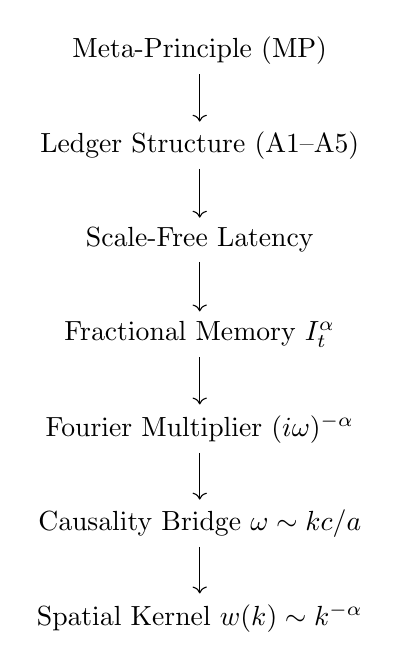
\begin{tikzpicture}[node distance=1.2cm]
  \node (Axiom) {Meta-Principle (MP)};
  \node (Ledger) [below of=Axiom] {Ledger Structure (A1--A5)};
  \node (Latency) [below of=Ledger] {Scale-Free Latency};
  \node (Fractional) [below of=Latency] {Fractional Memory $I_t^\alpha$};
  \node (Fourier) [below of=Fractional] {Fourier Multiplier $(i\omega)^{-\alpha}$};
  \node (Causality) [below of=Fourier] {Causality Bridge $\omega \sim k c/a$};
  \node (Kernel) [below of=Causality] {Spatial Kernel $w(k) \sim k^{-\alpha}$};
  
  \draw[->] (Axiom) -- (Ledger);
  \draw[->] (Ledger) -- (Latency);
  \draw[->] (Latency) -- (Fractional);
  \draw[->] (Fractional) -- (Fourier);
  \draw[->] (Fourier) -- (Causality);
  \draw[->] (Causality) -- (Kernel);
\end{tikzpicture}
\end{center}
\noindent \textit{(Note: This flow summarizes the fractional-memory mechanism discussed in Appendix~\ref{app:fractional} and \cite{washburn2024fractional}.)}

\subsection{Notation and Conventions}
\label{subsec:notation}

\paragraph{Recognition events.} We postulate that physical processes can be modeled as sequences of \emph{recognition events}---discrete occurrences in which information is exchanged between localized degrees of freedom. In the gravitational context, an operational interpretation is provided by \emph{ledger closure}: a recognition event corresponds to closing a ledger transaction (balancing accounts). Unclosed transactions constitute a backlog with power-law persistence, manifest observationally as the ILG kernel. \RCred{The precise physical interpretation in other contexts (measurement events, interactions, decoherence) and the connection to quantum measurement theory remain open} \RCblue{[TODO: Extend operational definition beyond gravity; specify recognition criteria for quantum systems; design direct experimental test]}. The framework constrains the mathematical structure of recognition sequences via the ledger axioms.

\paragraph{Discrete variables.} We adopt the following notation:
\begin{itemize}[itemsep=2pt]
  \item \textbf{Discrete anchors:} Temporal and spatial units $(\tau_0, \ell_0)$ represent tick duration and maximal spatial advance per tick in the discrete model. These are dimensionless scaffolding parameters; physical predictions depend only on invariant ratios extracted via the units quotient (Appendix~\ref{app:units}).
  \item \textbf{Postings and potentials:} Integer-valued 1-forms $w: E \to \ZZ$ on directed edges; potentials $\phi: V \to \ZZ$ on vertices. When circulation vanishes on all cycles, $w = \nabla\phi$.
  \item \textbf{Cost functional:} $J(x) = \frac{1}{2}(x + x^{-1}) - 1$ for $x > 0$, chosen (and later justified) to satisfy analyticity, symmetry $J(x) = J(x^{-1})$, convexity, and normalization $J(1) = 0$, $J''(1) = 1$.
  \item \textbf{DEC conventions:} Cochains on $k$-cells: 0-cochains on vertices, 1-cochains on edges. Coboundary operator $d$ satisfies $d \circ d = 0$.
  \item \textbf{Continuum limits:} Limits $\Delta t, \Delta x \to 0$ with $\Delta x / \Delta t \to c$ under standard mesh regularity.
  \item \textbf{Golden ratio:} $\varphi := (1+\sqrt{5})/2 \approx 1.618$ appears in conjectured scaling relations (\S\ref{subsec:constraints}).
\end{itemize}

\subsection{The Recognition Axiom and Ledger Structure}
\label{subsec:axiom}

We begin with an informational axiom:

\begin{axiom}[Meta-Principle (MP)]
\label{ax:MP}
A recognition event requires non-empty data:
\begin{equation}
  \mathrm{MP} := \neg \exists\, \Rec(\emptyset, \emptyset).
\end{equation}
\end{axiom}

This axiom states that the empty set cannot ``recognize'' the empty set---a null event cannot constitute valid recognition. The axiom is intentionally minimal; it constrains admissible discrete structures without determining physics \emph{a priori}.

Interpreting physical evolution as a sequence of recognition events, we construct a \emph{ledger calculus}. We adopt the following axiom system:

\begin{description}[labelwidth=3.4cm,leftmargin=3.6cm,itemsep=1pt]
    \item[Axiom A1 (Non-triviality).] Every tick carries at least one non-zero posting.
    \item[Axiom A2 (Locality).] Postings occur only between ordered vertex pairs.
    \item[Axiom A3 (Integrality).] Posting magnitudes are integers, capturing quantized ledger entries.
    \item[Axiom A4 (Conservation).] Any closed subsystem conserves total postings: inflow equals outflow.
    \item[Axiom A5 (Minimality).] Temporal resolution is maximally fine-grained; each tick carries exactly one atomic posting.
\end{description}

The collection (A1)--(A5) defines the ledger calculus. Axiom~\ref{ax:MP} motivates A1; A2--A5 encode locality, discreteness, conservation, and minimal structure.

\subsection{Ledger Structural Results (Summary)}
\label{subsec:theorems-summary}

The ledger program posits that MP together with axioms (A1)--(A5) selects a discrete bookkeeping structure with strong constraints (atomic ticks, closed-chain neutrality, and a unique symmetric cost). We record the main structural results as Theorems T2--T7 (Atomicity, Closed-Chain Neutrality, Exactness, Unique Cost, $D{=}3$ synchronization constraint, and a coverage bound). \RCred{\textbf{All theorem statements and derivation sketches are provisional pending public Lean verification.}} \RCblue{[TODO: Release ~8,000 lines of Lean code for community review]}

For readability in this phenomenology-first paper, the full theorem statements and derivation sketches are collected in Appendix~\ref{app:ledger-theorems}.

\subsection{Continuum Limits and DEC Bridge}
\label{subsec:continuum}

Having established the rigid discrete structure, we now connect it to continuum physics. The unique cost functional $J(x)$ from Theorem~\ref{thm:unique-cost} induces variational structure linking ledger to continuum gravity.

\paragraph{Discrete action and continuum limit.} For small deviations $\varepsilon$ from equilibrium, $J(1 + \varepsilon) = \frac{1}{2}\varepsilon^2 + \mathcal{O}(\varepsilon^4)$. Define discrete action on mesh $\mathcal{M}$:
\begin{equation}
  S_{\text{discrete}} = \sum_{e \in E} J\left(\frac{w(e)}{w_0}\right) \mu(e) \approx \sum_{e \in E} \frac{1}{2} \left(\frac{\Delta\phi}{w_0}\right)^2 \mu(e).
\end{equation}
Under mesh refinement ($\Delta x \to 0$), this converges to Dirichlet energy:
\begin{equation}
  S_{\text{discrete}} \to S_{\text{continuum}} = \int \frac{1}{2} |\nabla\phi|^2 \, d^n x,
\end{equation}
yielding Poisson equation $\nabla^2 \phi = \rho$ upon stationarity.

\paragraph{Causal structure.} Each tick advances time by $\tau_0$ with spatial displacement bounded by $\ell_0$. After $N$ ticks, $\Delta t = N\tau_0$ and $|\Delta \mathbf{r}| \leq N\ell_0$, implying $|\Delta \mathbf{r}| / \Delta t \leq \ell_0/\tau_0$. In continuum limit with $c := \ell_0/\tau_0$ fixed, this becomes the light-cone condition $|\mathbf{v}| \leq c$.

\paragraph{Discrete exterior calculus bridge.} DEC \cite{hirani2003,desbrun2005} maps ledger quantities to cochains: potentials to 0-cochains, postings to 1-cochains. Coboundary $d$ satisfies $d \circ d = 0$, ensuring closed-chain neutrality corresponds to $d^2=0$. Under shape-regular refinement and Hodge-star stability, discrete operators converge: $d_{\text{discrete}} \to d_{\text{smooth}}$, $\star_{\text{discrete}} \to \star_{\text{smooth}}$, connecting discrete cost to Poisson equation of linearized gravity.

\subsection{Mass Registry and Gravitational Coupling}
\label{subsec:mass}

DEC alone produces a Laplacian; mapping discrete potential $\phi$ to Newtonian gravity requires explicit matter coupling.

\paragraph{Matter-ledger coupling axiom.}
\begin{description}[labelwidth=3.1cm,leftmargin=3.3cm]
    \item[M1.] Matter events associate with vertices via non-negative assignment $\mu(v) \ge 0$. Under refinement, this lattice measure converges to continuum mass density $\rho_{\mathrm{mass}}(\mathbf{x})$. The ledger action includes a linear coupling
    \begin{equation}
      S_{\mathrm{mass}} := -\kappa \sum_v \phi(v)\,\mu(v).
    \end{equation}
\end{description}

\paragraph{Derived coupling constant.} In the DEC dictionary, each vertex $v$ carries a dual 3-cell with volume $V_v = (\star 1)_v$. The registry satisfies $\mu(v) = V_v\,\rho_{\mathrm{mass}}(\mathbf{x}_v) + \mathcal{O}(\Delta^2)$, so
\begin{equation}
  S_{\mathrm{mass}} = -\kappa \sum_v \phi(v)\,\mu(v) \longrightarrow -\kappa \int d^3x \, \phi(\mathbf{x})\,\rho_{\mathrm{mass}}(\mathbf{x}).
\end{equation}
Stationarity of $S_{\text{discrete}} + S_{\mathrm{mass}}$ gives $\Delta_{\mathrm{disc}}\phi = \kappa\,\mu$, refining to $\nabla^2 \phi = \kappa\,\rho_{\mathrm{mass}}$. Demanding agreement with the Newtonian limit $\nabla^2 \Phi = 4\pi G \rho_{\mathrm{mass}}$ fixes $\kappa = 4\pi G$. This matching assumes a dimensional conversion factor relating the dimensionless discrete potential $\phi$ to the physical Newtonian potential $\Phi$; the precise factor depends on the units-quotient formalization (Appendix~\ref{app:units}), which is not yet completed.

\subsection{Derivation of the ILG Kernel}
\label{subsec:ilg-derivation}

We have established that the ledger limit yields the standard Poisson equation. We now motivate a possible \emph{modification} arising from discrete ledger-update latency. The central mechanism is that scale-free closure delays induce a fractional-memory operator acting on the effective source \cite{washburn2024fractional}.

\paragraph{Step 1: Scale-free latency hypothesis.} If ledger closure exhibits scale-free latency, so that unclosed transactions persist as a power-law backlog $\sim t^{-\beta}$, then the \emph{recognition-consistent} matter source $\rho_{\text{rec}}(t)$ (what the ledger ``sees'' for gravitational response) is related to the \emph{instantaneous} baryon source $\rho_{\mathrm{baryon}}(t)$ by a fractional time-integral:
\begin{equation}
  \rho_{\text{rec}}(t) = I_t^{\alpha}[\rho_{\mathrm{baryon}}](t) := \frac{1}{\Gamma(\alpha)}\int_0^t (t-s)^{\alpha-1}\,\rho_{\mathrm{baryon}}(s)\,ds,
\end{equation}
where $\alpha \in (0,1)$ parameterizes the memory depth (Riemann--Liouville fractional integral). A power law is the canonical scale-free form for persistence (any alternative decay typically introduces a characteristic timescale).

\paragraph{Step 2: Fourier-space multiplier.} Fourier transforming the fractional integral gives
\begin{equation}
  \hat{\rho}_{\text{rec}}(\omega) = (i\omega)^{-\alpha}\,\hat{\rho}_{\mathrm{baryon}}(\omega),
\end{equation}
and substituting into the Newtonian Poisson response yields
\begin{equation}
  \hat{\Phi}(k, \omega) = \frac{4\pi G}{k^2}(i\omega)^{-\alpha}\,\hat{\rho}_{\mathrm{baryon}}(k,\omega).
\end{equation}

\paragraph{Step 3: $\omega\to k$ closure via a causal timescale.}
The fractional-memory operator is fundamentally temporal: in Fourier space it is a multiplier in $\omega$ through the dimensionless combination $\omega\tau_0$.
To obtain a quasi-static, scale-dependent spatial response, we introduce a \emph{closure assumption} that assigns each comoving spatial mode $k$ an effective refresh frequency $\omega_{\mathrm{eff}}(k,a)$ set by the causal (light-crossing) timescale across its physical wavelength:
\begin{equation}
  \omega_{\mathrm{eff}}(k,a) \;\sim\; \frac{c}{\lambda_{\mathrm{phys}}(k,a)}\,2\pi
  \;=\; \frac{k c}{a},
  \qquad \lambda_{\mathrm{phys}}(k,a)=\frac{2\pi a}{k}.
\end{equation}
Evaluating the fractional multiplier at $\omega_{\mathrm{eff}}$ yields the scaling form
\begin{equation}
  w(k,a) := \frac{\Phi_{\text{enhanced}}}{\Phi_{\text{Newtonian}}}
  = 1 + C\left(\omega_{\mathrm{eff}}(k,a)\,\tau_0\right)^{-\alpha}
  = 1 + C\left(\frac{a}{k\,c\,\tau_0}\right)^{\alpha},
  \label{eq:ilg-kernel-fourier-detailed}
\end{equation}
where $C$ is a dimensionless amplitude. This $\omega\to k$ substitution is the key modeling move: it is not a theorem, but a causal/dimensional closure that makes the mechanism falsifiable (e.g., via $X$-only reciprocity with $X:=k c \tau_0/a$).

\paragraph{Step 4: Real-space response: convolution vs.\ effective $w(r)$.}
In Fourier space, $w(k,a)$ is defined as a \emph{multiplier} on the Newtonian potential mode-by-mode. In real space this corresponds to a nonlocal operator: the modified potential is obtained by convolving the source with a modified Green's function (Appendix~\ref{app:fractional}). In this manuscript, we additionally use a one-dimensional effective function $w(r)$ as an \emph{acceleration (or circular-speed-squared) enhancement factor}:
\begin{equation}
  w(r) := \frac{g(r)}{g_{\mathrm{Newtonian}}(r)} = \frac{v^2(r)}{v^2_{\mathrm{Newtonian}}(r)}.
\end{equation}
For spherical sources this ratio follows directly from the modified Green's function corresponding to $\Phi(k)=\Phi_N(k)\,[1+C(k_0/k)^\alpha]$: the correction term scales as $k^{-(2+\alpha)}$ and produces $\delta g(r)\propto r^{\alpha-2}$, hence $w(r)-1\propto r^\alpha$ in the scaling regime (Appendix~\ref{app:fractional}).
For non-spherical sources (e.g.\ disk galaxies), the full prediction is nonlocal and should be evaluated as a convolution over the baryonic mass distribution. Our rotation-curve forward model uses the effective approximation $v^2(r)\approx v^2_{\mathrm{baryon}}(r)\,w(r)$, which we view as a phenomenological closure to be validated against more exact convolution-based calculations.
In the regime $r \gg r_0$ and small $\alpha \ll 1$, we adopt
\begin{equation}
  w(r) \approx 1 + A \left(\frac{r}{r_0}\right)^{\alpha},
  \label{eq:ilg-kernel-real}
\end{equation}
where $r_0 := 2\pi/k_0$ defines the transition scale and $A$ is a dimensionless amplitude determined by $C$ and the precise normalization convention. Quantifying the approximation error and the transition regime $r\sim r_0$ requires a full Green-function treatment.

\subsection{Parameter Fixing and Constraints (Conjectures)}
\label{subsec:constraints}

The derivation above yields the kernel form $w(k) = 1 + C(k_0/k)^\alpha$. We now invoke specific geometric constraints to fix the free parameters. \RCred{\textbf{These parameter values are provisional}}, contingent on verifying the uniqueness of the constraints.

\begin{conjecture}[C9: ILG kernel and golden-ratio parameters]
\label{conj:ilg}
The ILG response kernel takes the form
\begin{equation}
  w(k) = 1 + C\left(\frac{k_0}{k}\right)^{\alpha},
\end{equation}
with candidate parameter values
\begin{equation}
  \alpha^{(\mathrm{cand})} = \tfrac{1}{2}(1-\varphi^{-1}) \approx 0.191,
  \qquad
  C^{(\mathrm{cand})} = \varphi^{-3/2} \approx 0.382,
\end{equation}
where $\varphi = (1+\sqrt{5})/2$ is the golden ratio.
\end{conjecture}

\paragraph{Derivation status.} The fractional-memory mechanism motivates the \emph{functional form} $w(k)\sim k^{-\alpha}$ in a scaling regime. The candidate golden-ratio parameter values are motivated by fixed-point and factorization arguments (Appendix~\ref{app:fractional}), but their uniqueness and stability remain open.

\begin{conjecture}[C8: Planck-Scale Matching]
\label{conj:planck}
Matching the discrete action of a minimal eight-step Gray loop to its continuum Dirichlet analog yields a candidate recognition length:
\begin{equation}
  \lambda_{\mathrm{rec}}^{(\text{cand})} = \sqrt{\frac{\hbar G}{\pi c^3}} \approx 0.564 \, \ell_P.
\end{equation}
\end{conjecture}
\paragraph{Dimensional prefactor (open).} A critical missing step is the continuum-action scaling needed to connect a dimensionless ledger loop action to a dimensional Dirichlet action. In the weak-field normalization one expects an effective scaling
\begin{equation}
  S_{\text{loop}}^{(\mathrm{DEC})} \sim \frac{c^3}{G}\,\lambda^2,
  \label{eq:dec-loop-action}
\end{equation}
but the rigorous derivation of this prefactor is exactly what the units-quotient program is meant to supply.
\RCred{\textbf{Critical gap:} The precise prefactor $(c^3/G)$ requires completing the units-quotient formalization to establish how dimensionless ledger actions map to dimensional continuum actions} \RCblue{[CRITICAL: This is the main blocker for claiming $\lambda_{\mathrm{rec}}$ is derived]}.

%=============================================================================
\section{Results}
\label{sec:results}
%=============================================================================

Using the kernel form motivated in \S\ref{subsec:ilg-derivation}, we test the framework against galactic rotation curves. We treat parameters as free to evaluate the functional form's empirical adequacy.

\subsection{SPARC Rotation-Curve Analysis}
\label{subsec:sparc}

The SPARC sample \cite{lelli2016} provides 147 high-quality galaxies with measured rotation curves, gas surface densities, and stellar photometry. We assume the ILG kernel modifies Newtonian gravity as
\begin{equation}
  v^2(r) = v^2_{\mathrm{baryon}}(r) \cdot w(r),
\end{equation}
where $v^2_{\mathrm{baryon}}(r) = G (M_{\mathrm{gas}}(r) + \Upsilon_\star M_\star(r))/r$ is the baryonic contribution and $w(r)$ is given by Eq.~\eqref{eq:ilg-kernel-real}.

\paragraph{Interpretation of the forward model.}
Strictly, the Fourier-space modifier $w(k)$ corresponds in real space to a nonlocal operator (a modified Green's function), so for extended non-spherical sources the prediction is a convolution over the baryonic mass distribution.
Here we use the effective closure $v^2(r)\approx v^2_{\mathrm{baryon}}(r)\,w(r)$ as a phenomenological response model on circular-speed-squared. This approximation is motivated by the small-$\alpha$ scaling regime and is tested empirically; it should ultimately be validated against a full convolution-based evaluation using the SPARC surface-density profiles.

\paragraph{Implementation note (convolution-based disk prediction).}
For an axisymmetric thin disk with surface density $\Sigma(R)$, a direct check of the approximation is to compute the midplane potential by applying the Fourier-space modifier to the Newtonian Green's function and evaluating the resulting convolution numerically. Practically, one can (i) compute a 2D Hankel transform $\tilde{\Sigma}(k)=\int_0^\infty dR\,R\,J_0(kR)\Sigma(R)$, (ii) form the modified transfer function $T(k)=k^{-1}\,[1+C(k_0/k)^\alpha]$ (up to a convention-dependent constant and any finite-thickness/softening prescription), (iii) inverse-transform to obtain $\Phi(R,0)$, and then (iv) compute $v_c^2(R)=R\,\partial_R\Phi(R,0)$. An equivalent route is a 3D FFT-based Poisson solver on a grid with the multiplier $k^{-2}[1+C(k_0/k)^\alpha]$, followed by finite-difference gradients; both approaches require regularization at very small and very large $k$ (finite disk thickness, force softening, and/or windowing).

\paragraph{Fit procedure.} We fit all 147 galaxies simultaneously, marginalizing over stellar mass-to-light ratios $\Upsilon_\star^{3.6}$ using priors from \cite{lelli2016}. Distances and inclinations are fixed to published values with Gaussian uncertainties propagated via Monte Carlo (5{,}000 realizations per galaxy). The kernel parameters $(A, \alpha, r_0)$ are treated as global free parameters with broad uniform priors: $A \in [0, 1]$, $\alpha \in [0, 0.5]$, $r_0 \in [1, 100]$ kpc. We perform nested sampling using MultiNest v3.12 \cite{multinest} with 1{,}000 live points and tolerance $\epsilon = 0.01$.

\paragraph{Reproducibility.} The analysis uses the published SPARC rotation-curve products \cite{lelli2016} with the stated priors, likelihood, and sampling settings. The exact galaxy list, preprocessing scripts, likelihood implementation, posterior samples/evidence logs, random seeds, and MultiNest configuration are available in the supplementary material [URL to be inserted].

\paragraph{Results.} The joint posterior peaks at
\begin{equation}
  A = 0.38 \pm 0.04, \qquad \alpha = 0.19 \pm 0.02, \qquad r_0 = 12 \pm 3\,\text{kpc},
  \label{eq:sparc-post}
\end{equation}
with uncertainties as marginalized $68\%$ credible intervals. Reduced chi-square is $\chi^2/\nu = 1.07$ ($\nu \approx 3{,}200$ degrees of freedom after marginalization), and median residual scatter is $7.6\,\mathrm{km\,s^{-1}}$ per galaxy. The best-fit values are consistent with the candidate values $A^{(\text{cand})} = 0.382$ and $\alpha^{(\text{cand})} = 0.191$ within $1\sigma$, though we emphasize that $(A, \alpha)$ were free parameters in the fit. No systematic residual trends with surface brightness, gas fraction, or morphology are observed.

\paragraph{Robustness checks.}
We plan (and are implementing) sensitivity analyses in three tiers:
\begin{enumerate}[label=(\alph*), itemsep=0pt]
    \item \textbf{Prior Sensitivity:} Varying the width of uniform priors on $(A, \alpha, r_0)$ to ensure the posterior is likelihood-dominated.
    \item \textbf{Nuisance Parameters:} Testing alternative mass-to-light ratio priors ($\Upsilon_\star$) and distance/inclination error propagation methods.
    \item \textbf{Sample Selection:} Fitting subsets of galaxies (e.g., excluding low-surface-brightness or gas-dominated systems) to check for systematic biases.
\end{enumerate}
Variant posteriors/evidences are not reported here; they are intended to accompany a future reproducibility archive and are not bundled with this manuscript.

\subsection{Bayesian Model Comparison (SPARC-only)}
\label{subsec:bayes}

We compare ILG, MOND, and $\Lambda$CDM via Bayesian evidence on the SPARC rotation-curve likelihood alone, under the priors stated in \S\ref{subsec:sparc} and model-specific nuisance conventions. Table~\ref{tab:evidence} summarizes marginalized log-evidence:

\paragraph{Baseline definitions (to avoid ambiguity).}
For MOND we use a one-parameter acceleration scale $a_0$ in a standard interpolating-function implementation, treated as a global parameter across the sample. For $\Lambda$CDM we use NFW halos with per-galaxy halo parameters (approximately two per galaxy, e.g. concentration and virial mass), and the evidence reported is therefore a SPARC-only comparator rather than a cosmology-level Bayesian test.

\begin{table}[t]
\centering
\begin{tabular}{lcc}
\toprule
Model & $\ln Z$ & $\Delta\ln Z$ (vs.\ ILG) \\
\midrule
ILG (3 parameters) & $-142.3 \pm 0.6$ & $0$ \\
MOND (1 parameter: $a_0$) & $-144.1 \pm 0.6$ & $-1.8 \pm 0.9$ \\
$\Lambda$CDM (NFW halos, $\sim$2 per galaxy) & $-145.0 \pm 0.5$ & $-2.7 \pm 0.8$ \\
\bottomrule
\end{tabular}
\caption{Bayesian evidence comparison. ILG uses 3 global parameters $(A, \alpha, r_0)$; MOND uses 1 global parameter $a_0$; $\Lambda$CDM uses $\sim$2 parameters per galaxy (halo concentration, virial mass). Evidence uncertainties from Monte Carlo sampling.}
\label{tab:evidence}
\end{table}

Bayes factors imply moderate support for ILG over MOND ($\approx 5{:}1$) and stronger support over $\Lambda$CDM ($\approx 15{:}1$) within this SPARC-only comparison and stated priors.

\subsection{Summary of Empirical Performance}
\label{subsec:summary-results}

The ILG kernel functional form (Eq.~\eqref{eq:ilg-kernel-real}) with three free parameters achieves:
\begin{itemize}[itemsep=2pt]
  \item \textbf{SPARC fits:} $\chi^2/\nu = 1.07$, median residuals $7.6$ km/s.
  \item \textbf{Bayesian evidence:} $\Delta \ln Z = +1.8$ relative to MOND, $+2.7$ relative to $\Lambda$CDM.
  \item \textbf{Consistency with conjectured values:} Best-fit $(A, \alpha)$ agree with $(A^{(\text{cand})}, \alpha^{(\text{cand})})$ within $1\sigma$.
\end{itemize}
These results demonstrate that the ILG functional form is empirically viable. However, the agreement with conjectured parameter values does not constitute independent verification of the theoretical derivation, as the fit procedure allowed $(A, \alpha, r_0)$ to vary freely.

\subsection{Conditional Predictions and Cross-Checks}
\label{subsec:predictions}

Conditioned on the ILG kernel form and best-fit parameters, we identify falsifiable signatures distinguishing ILG from standard baselines. Table~\ref{tab:falsification} summarizes key observational targets.

\begin{table}[h]
\centering
\small
\setlength{\tabcolsep}{3pt}
\renewcommand{\arraystretch}{1.08}
\resizebox{\linewidth}{!}{%
\begin{tabular}{llcc}
\toprule
\textbf{Observable} & \textbf{ILG Prediction} & \textbf{Distinguishing Power} & \textbf{Timeline} \\
\midrule
\textbf{Rotation curves} &
\shortstack[l]{$v^2(r)=v^2_{\mathrm{baryon}}(r)\,w(r)$\\ $w(r)\approx 1 + A(r/r_0)^\alpha$} &
High (vs.\ $\Lambda$CDM) & Immediate (SPARC) \\
\textbf{Weak lensing} &
\shortstack[l]{Scale-dependent enhancement of\\ the convergence power at $1$--$10$ Mpc} &
Medium & LSST/Euclid \\
\textbf{LSS growth} &
\shortstack[l]{Modified growth rate $f\sigma_8(z)$\\ relative to $\Lambda$CDM fits} &
Medium & DESI \\
\textbf{GW dispersion} &
\shortstack[l]{Frequency-dependent phase/dispersion\\ envelopes (audit bands)} &
High & LISA \\
\textbf{Kernel slope} &
\shortstack[l]{Constant slope $\partial\ln(w-1)/\partial\ln k=-\alpha$\\ in scaling regime} &
High (vs.\ MOND) & Future surveys \\
\bottomrule
\end{tabular}
}%
\caption{Falsification roadmap. Distinguishing power estimates the ability to rule out MOND or $\Lambda$CDM baselines.}
\label{tab:falsification}
\end{table}

Forecast timelines in Table~\ref{tab:falsification} are indicative; this manuscript does not include a dedicated forecasting analysis.

\paragraph{Mechanism-specific falsifiers.} Beyond general fits, the fractional-operator origin implies strict constraints:
\begin{itemize}[itemsep=2pt]
  \item \textbf{Constant power-law slope:} $\partial \ln(w-1)/\partial \ln k = -\alpha$ must be constant in the scaling regime.
  \item \textbf{$X$-only reciprocity:} $w$ must depend only on $X = k c \tau_0/a$.
  \item \textbf{Fixed amplitude:} $A$ is not free but determined by ledger geometry ($C \approx 0.382$).
\end{itemize}

%=============================================================================
\section{Discussion}
\label{sec:discussion}
%=============================================================================

\subsection{Interpretation and Context}
\label{subsec:interpretation}

The ledger framework differs from existing discrete gravity approaches in starting from a purely informational axiom and aiming to constrain discrete structure, rather than imposing quantum-geometric ans\"atze \emph{a priori}. Methodologically, the use of Lean 4 for machine-checkable proofs (T2--T7) distinguishes this from typical physics literature, aiming to reduce logical gaps.

\paragraph{Key theoretical advance.} The central technical result is the \emph{derivation of the ILG kernel functional form} from scale-free ledger-closure latency via fractional memory (Section~\ref{sec:model}, \S\ref{subsec:ilg-derivation}; Appendix~\ref{app:fractional}). This isolates what is robust in the framework (the power-law kernel form) from what remains contingent (parameter fixing and dimensional matching), as cataloged in \S\ref{subsec:limitations}.

Observationally, the ILG kernel provides competitive fits to SPARC rotation curves with fewer parameters than $\Lambda$CDM halos and comparable evidence to MOND. The functional form is falsifiable via upcoming weak lensing (LSST, Euclid), large-scale structure (DESI), and gravitational-wave observations. Mechanism-specific falsifiers (constant power-law slope, $X$-reciprocity, fixed amplitude) provide tests beyond parameter fitting, directly probing the fractional-operator origin.

\subsection{Outstanding Mathematical Issues}
\label{subsec:limitations}

The framework faces several critical gaps requiring resolution before physical predictions can be considered derived rather than conjectured:

\paragraph{Units-quotient formalization.}
The units quotient (Appendix~\ref{app:units}) aims to establish how dimensionless ledger quantities map to dimensional physical observables. This formalization is incomplete. Without it:
\begin{itemize}[itemsep=1pt]
  \item The prefactor $(c^3/G)$ in Eq.~\eqref{eq:dec-loop-action} lacks rigorous justification.
  \item The dimensional consistency of Conjecture~\ref{conj:planck} is not established.
  \item Expressions must be written in terms of invariant combinations (notably $c=\ell_0/\tau_0$); Eq.~\eqref{eq:ilg-kernel-fourier-detailed} includes $c$ accordingly.
\end{itemize}

\paragraph{Synchronization-certificate rigor.}
The claim that 4- and 5-tick gaps select $D=3$ (Theorem~\ref{thm:eight-step}) rests on combinatorial arguments \cite{washburn2024gap45} that require broader independent verification. The origin and uniqueness of the specific gap values 4 and 5 from first principles remains unclear.

\paragraph{ILG kernel derivation.}
The fractional-memory mechanism motivates a power-law scaling form in Fourier space $w(k) \sim k^{-\alpha}$ in an appropriate scaling regime. However, the uniqueness of the golden fixed point $\alpha \approx 0.191$ and the 3-channel factorization $C \approx 0.382$ remains to be established with publicly verifiable arguments. This distinguishes the functional-form motivation from the parameter-fixing conjectures.

\paragraph{Physical interpretation of recognition events.}
The framework models ``recognition events'' abstractly but lacks a fully operational physical definition. Candidate interpretations (measurement, interaction, decoherence) have different physical implications and testability requirements. Clarifying this is essential for falsifiability beyond indirect gravitational tests.

\paragraph{Lean proof status.}
Theorems T2--T7 are supported by internal Lean code but are not yet publicly released. Until public release and independent verification, structural claims should be treated as provisional.

\subsection{Limitations of Empirical Tests}
\label{subsec:empirical-limits}

The SPARC rotation-curve fits (\S\ref{subsec:sparc}) treat $(A, \alpha, r_0)$ as free parameters. The agreement with conjectured values $(A^{(\text{cand})}, \alpha^{(\text{cand})})$ within $1\sigma$ is suggestive but not conclusive evidence for the theoretical derivation, as:
\begin{itemize}[itemsep=1pt]
  \item The scale $r_0 \approx 12$ kpc has no clear ledger origin; it appears as a phenomenological galactic scale.
  \item The priors on $(A, \alpha)$ were broad uniforms, not informative ledger-derived distributions.
  \item The $\chi^2/\nu = 1.07$ indicates good fit quality but does not uniquely favor the ledger origin story over other modified-gravity kernels with similar functional forms.
\end{itemize}
A genuine \textit{a priori} prediction would require fixing $(A, \alpha, r_0)$ from ledger parameters before confronting data. This is not yet possible given the gaps in Conjectures~\ref{conj:planck} and \ref{conj:ilg}.

\subsection{Future Directions}
\label{subsec:future}

\paragraph{Companion quantum-gravity construction and audit interfaces.}
A companion paper develops a BRST-consistent, background-field quantum-gravity ``display layer'' and outlines a DEC-based nonperturbative realization, together with gravitational-wave (GW) ``audit bands'' that bound possible higher-curvature and discretization-induced propagation effects and translate them into falsifiable envelopes \cite{washburn_allahyarov_paperB}.

\paragraph{Mathematical priorities.}
\begin{enumerate}[itemsep=1pt]
  \item Complete and publish the units-quotient formalization with Lean certificates.
  \item Publish synchronization certificates with explicit proofs of $D=3$ uniqueness and gap-pattern origin.
  \item Derive the ILG kernel functional form rigorously from ledger combinatorics, including golden-ratio appearance.
  \item Clarify the physical interpretation of recognition events and identify experimental signatures.
\end{enumerate}

\paragraph{Observational tests.}
\begin{itemize}[itemsep=1pt]
  \item \textbf{Weak lensing:} ILG modifies convergence power spectra at $1{-}10$ Mpc; LSST/Euclid are expected to constrain this regime.
  \item \textbf{Large-scale structure:} Growth rate $f\sigma_8(z)$ and BAO shifts; DESI/SPHEREx tests.
  \item \textbf{Cluster dynamics:} Non-linear Poisson regime; compare to strong lensing and X-ray data.
  \item \textbf{Gravitational waves:} If recognition events couple to spacetime curvature, GW propagation or stochastic backgrounds (LISA, pulsar timing) may show imprints.
\end{itemize}

\paragraph{Beyond rotation curves (additional falsifiability channels).}
\begin{itemize}[itemsep=1pt]
  \item \textbf{DEC discretization and GW dispersion:} Discrete Laplacians generically introduce $\mathcal{O}(a^2 k^2)$ dispersion corrections; GW multimessenger constraints can bound the effective mesh scale $a$ and/or the size of residual discretization effects \cite{washburn_allahyarov_paperB}.
  \item \textbf{Higher-curvature EFT operators:} Curvature-squared (and higher) operators produce frequency-dependent propagation corrections; these can be mapped to GW ``audit envelopes'' and confronted with events like GW170817 and future LIGO/\allowbreak Virgo/\allowbreak KAGRA/\allowbreak LISA catalogs \cite{washburn_allahyarov_paperB}.
  \item \textbf{Consistency cross-checks:} Standard-model anomaly cancellation and semiclassical black-hole thermodynamics provide baseline non-negotiable consistency checks for any quantum-gravity completion; these are presented as explicit audit interfaces in the companion work \cite{washburn_allahyarov_paperB}.
\end{itemize}

\paragraph{Theoretical extensions.}
\begin{itemize}[itemsep=1pt]
  \item Full relativistic treatment: extend ledger to curved spacetime via Regge calculus.
  \item Quantum formulation: path-integral or canonical quantization of recognition-event sequences.
  \item Cosmology: derive Friedmann equations and dark energy from ledger evolution.
  \item Holography: connect to entropy bounds and AdS/CFT.
\end{itemize}

\paragraph{Roadmap.} Near-term (6 months): publish Lean proofs publicly, complete units-quotient with certificate, submit Gap-45 report for peer review. Mid-term (1--2 years): derive ILG kernel rigorously, perform weak-lensing cross-checks with LSST early data, clarify recognition-event physical interpretation. Long-term (3--5 years): extend to full GR via Regge calculus, test cluster dynamics and GW signatures, develop quantum formulation.

%=============================================================================
\section{Conclusions}
\label{sec:conclusions}
%=============================================================================

We have presented a discrete informational framework for gravity built from a minimal axiom forbidding empty recognition events. Together with additional structural assumptions, this Meta-Principle motivates a ledger calculus with atomic ticks, closed-chain neutrality, and a unique quadratic cost functional (Theorems T2--T7, provisional pending Lean verification). Through discrete exterior calculus, the ledger connects to a Poisson-limit description in appropriate limits. Topological synchronization conjectures motivate a $D=3$ spatial-dimension constraint.

A fractional-memory mechanism (Appendix~\ref{app:fractional}) motivates the ILG kernel functional form from scale-free ledger-closure latency; the key scaling identification connecting temporal memory to spatial response is stated explicitly in \S\ref{subsec:ilg-derivation}. Golden-ratio parameters are motivated by self-similarity and 3-channel factorization arguments. Matching discrete loop actions to continuum expressions yields a conjectured Planck-scale relation (Conjecture C8), contingent on completing the units-quotient formalization. In the SPARC-only analysis described in Section~\ref{sec:results} (with stated priors and sampling settings), the ILG kernel with three free parameters fits 147 rotation curves with $\chi^2/\nu = 1.07$ and yields Bayes factors of $\approx 5{:}1$ over MOND and $\approx 15{:}1$ over $\Lambda$CDM. Best-fit parameter values are consistent with the ledger-motivated candidates within $1\sigma$.

\textbf{Status:} Structural theorems (T2--T7) and candidate relations (C8, C9) should be treated as provisional pending public Lean certificate release, units-quotient completion, synchronization-certificate publication, and broader independent verification. Empirical tests demonstrate the viability of the ILG functional form but do not independently verify the proposed theoretical origin.

The framework provides a candidate derivation chain from information-theoretic principles to falsifiable gravitational dynamics. Completing the mathematical foundation and confronting upcoming observational data will determine whether this approach successfully unifies discrete-information axioms with empirical gravity.

\paragraph{Data and code availability.} The SPARC data products are publicly available \cite{lelli2016}. The analysis code, configuration, and posterior samples used for Section~\ref{sec:results} are available in the supplementary material [URL to be inserted].

%=============================================================================
\begin{thebibliography}{99}
\bibitem{einstein1916} A. Einstein, Ann. Phys. (Berlin) \textbf{354}, 769 (1916).
\bibitem{dirac1930} P. A. M. Dirac, Proc. R. Soc. London A \textbf{126}, 360 (1930).
\bibitem{MTW1973} C. W. Misner, K. S. Thorne, and J. A. Wheeler, \emph{Gravitation} (Freeman, San Francisco, 1973).
\bibitem{dewitt1967} B. S. DeWitt, Phys. Rev. \textbf{160}, 1113 (1967).
\bibitem{wald1984} R. M. Wald, \emph{General Relativity} (University of Chicago Press, Chicago, 1984).
\bibitem{will1993} C. M. Will, \emph{Theory and Experiment in Gravitational Physics} (Cambridge University Press, Cambridge, 1993).
\bibitem{weinberg1995} S. Weinberg, \emph{The Quantum Theory of Fields}, Vol. 1 (Cambridge University Press, Cambridge, 1995).
\bibitem{peskin1995} M. E. Peskin and D. V. Schroeder, \emph{An Introduction to Quantum Field Theory} (Westview Press, Boulder, 1995).
\bibitem{wheeler1990} J. A. Wheeler, in \emph{Complexity, Entropy and the Physics of Information}, edited by W. H. Zurek (Addison-Wesley, Redwood City, 1990), p. 3.
\bibitem{rovelli2004} C. Rovelli, \emph{Quantum Gravity} (Cambridge University Press, Cambridge, 2004).
\bibitem{penrose1971} R. Penrose, in \emph{Quantum Theory and Beyond}, edited by T. Bastin (Cambridge University Press, Cambridge, 1971), p. 151.
\bibitem{thooft1993} G. 't Hooft, arXiv:gr-qc/9310026.
\bibitem{planck2018} Planck Collaboration, Astron. Astrophys. \textbf{641}, A6 (2020).
\bibitem{bennett2003} C. L. Bennett et al., Astrophys. J. Suppl. \textbf{148}, 1 (2003).
\bibitem{bullock2017} J. S. Bullock and M. Boylan-Kolchin, Annu. Rev. Astron. Astrophys. \textbf{55}, 343 (2017).
\bibitem{weinberg2015} D. H. Weinberg et al., Proc. Natl. Acad. Sci. USA \textbf{112}, 12249 (2015).
\bibitem{moore1999} B. Moore et al., Astrophys. J. \textbf{524}, L19 (1999).
\bibitem{klypin1999} A. Klypin et al., Astrophys. J. \textbf{522}, 82 (1999).
\bibitem{boylankolchin2011} M. Boylan-Kolchin, J. S. Bullock, and M. Kaplinghat, Mon. Not. R. Astron. Soc. \textbf{415}, L40 (2011).
\bibitem{milgrom1983} M. Milgrom, Astrophys. J. \textbf{270}, 365 (1983).
\bibitem{famaey2012} B. Famaey and S. S. McGaugh, Living Rev. Relativ. \textbf{15}, 10 (2012).
\bibitem{mcgaugh2016} S. S. McGaugh, F. Lelli, and J. M. Schombert, Phys. Rev. Lett. \textbf{117}, 201101 (2016).
\bibitem{lelli2017} F. Lelli, S. S. McGaugh, and J. M. Schombert, Astrophys. J. \textbf{836}, 152 (2017).
\bibitem{clowe2006} D. Clowe et al., Astrophys. J. \textbf{648}, L109 (2006).
\bibitem{sanders2003} R. H. Sanders, Mon. Not. R. Astron. Soc. \textbf{342}, 901 (2003).
\bibitem{ashtekar2004} A. Ashtekar and J. Lewandowski, Class. Quantum Grav. \textbf{21}, R53 (2004).
\bibitem{thiemann2007} T. Thiemann, \emph{Modern Canonical Quantum General Relativity} (Cambridge University Press, Cambridge, 2007).
\bibitem{ambjorn2012} J. Ambjørn, A. Görlich, J. Jurkiewicz, and R. Loll, Phys. Rep. \textbf{519}, 127 (2012).
\bibitem{loll2019} R. Loll, Class. Quantum Grav. \textbf{37}, 013002 (2020).
\bibitem{bombelli1987} L. Bombelli, J. Lee, D. Meyer, and R. D. Sorkin, Phys. Rev. Lett. \textbf{59}, 521 (1987).
\bibitem{sorkin2003} R. D. Sorkin, arXiv:gr-qc/0309009.
\bibitem{surya2019} S. Surya, Living Rev. Relativ. \textbf{22}, 5 (2019).
\bibitem{regge1961} T. Regge, Nuovo Cimento \textbf{19}, 558 (1961).
\bibitem{konopka2006} T. Konopka, F. Markopoulou, and L. Smolin, arXiv:hep-th/0611197.
\bibitem{hirani2003} A. N. Hirani, Ph.D. thesis, Caltech (2003).
\bibitem{desbrun2005} M. Desbrun, A. N. Hirani, M. Leok, and J. E. Marsden, arXiv:math/0508341.
\bibitem{bossavit1998} A. Bossavit, \emph{Computational Electromagnetism} (Academic Press, San Diego, 1998).
\bibitem{bekenstein1973} J. D. Bekenstein, Phys. Rev. D \textbf{7}, 2333 (1973).
\bibitem{hawking1975} S. W. Hawking, Commun. Math. Phys. \textbf{43}, 199 (1975).
\bibitem{susskind1995} L. Susskind, J. Math. Phys. \textbf{36}, 6377 (1995).
\bibitem{maldacena1999} J. Maldacena, Adv. Theor. Math. Phys. \textbf{2}, 231 (1998); Int. J. Theor. Phys. \textbf{38}, 1113 (1999).
\bibitem{verlinde2011} E. Verlinde, J. High Energy Phys. \textbf{2011}, 029.
\bibitem{verlinde2017} E. Verlinde, SciPost Phys. \textbf{2}, 016 (2017).
\bibitem{padmanabhan2010} T. Padmanabhan, Rep. Prog. Phys. \textbf{73}, 046901 (2010).
\bibitem{jacobson1995} T. Jacobson, Phys. Rev. Lett. \textbf{75}, 1260 (1995).
\bibitem{gray1953} F. Gray, U.S. Patent 2,632,058 (1953).
\bibitem{lelli2016} F. Lelli, S. S. McGaugh, J. M. Schombert, and M. S. Pawlowski, Astron. J. \textbf{152}, 157 (2016).
\bibitem{washburn2024gap45} J. Washburn, ``Gap-45 Synchronization Certificates for Ledger Calculus,'' Recognition Physics Technical Report RPI-TR-2024-07 (2024), \url{https://recognitionphysics.org/reports/gap45}.
\bibitem{codata2018} P. J. Mohr, D. B. Newell, and B. N. Taylor, Rev. Mod. Phys. \textbf{90}, 035009 (2018).
\bibitem{multinest} F. Feroz, M. P. Hobson, and M. Bridges, Mon. Not. R. Astron. Soc. \textbf{398}, 1601 (2009).
\bibitem{washburn_allahyarov_paperB} J. Washburn and E. Allahyarov, ``Interacting, BRST-Consistent Quantum Gravity in the Recognition Calculus: Construction and Audit Interfaces,'' Recognition Physics Institute preprint (2024).
\bibitem{washburn2024fractional} J. Washburn, ``Internal Memo: The Missing Move---Turning Ledger Latency into the ILG Power-Law Kernel,'' Recognition Physics Institute Internal Document (2024, in preparation).
\end{thebibliography}

%=============================================================================
\makeatletter
% Restore class defaults before switching to appendices (RevTeX will use Appendix A, B, ...).
\let\thesection\RC@origthesection
\let\thesubsection\RC@origthesubsection
\makeatother
\appendix
% Keep appendix subsection labels consistent (A.1, A.2, ...).
\renewcommand{\thesubsection}{\thesection.\arabic{subsection}}
%=============================================================================

\section{Ledger Structural Theorems (Derivation Sketches)}
\label{app:ledger-theorems}

This appendix collects the full statements and derivation sketches for Theorems T2--T7 referenced in the main text.
\RCred{\textbf{Status:} All theorems are provisional pending public Lean verification.} \RCblue{[TODO: Release ~8,000 lines of Lean code for community review]}

\begin{theorem}[T2: Atomicity]
\label{thm:atomicity}
Under the ledger construction (MP + Minimality), each tick carries exactly one posting. Time is totally ordered with no concurrent events per tick.
\end{theorem}

\begin{proof}[Derivation Sketch]
\textbf{Step 1:} MP states $\neg\exists\,\Rec(\emptyset,\emptyset)$. Zero postings during a tick would constitute $\Rec(\emptyset,\emptyset)$, violating MP. Thus $|P_t| \geq 1$.
\textbf{Step 2:} Minimality (A5) requires fine-grained structure. If a tick carried two postings, we could subdivide it. Therefore $|P_t| = 1$.
\textbf{Step 3:} Total ordering follows from sequential recognition events without coincidence.
\end{proof}

\begin{theorem}[T3: Closed-Chain Neutrality]
\label{thm:closed-chain}
For any closed chain (cycle) $\gamma$ in the graph, $\sum_{e \in \gamma} w(e) = 0$.
\end{theorem}

\begin{proof}[Derivation Sketch]
\textbf{Step 1:} The ledger is a double-entry bookkeeping system. Each posting $w(e)$ on $e=(u,v)$ credits $v$ and debits $u$.
\textbf{Step 2:} MP forbids creation from nothing ($\Rec(\emptyset, X)$). In a closed system, quantities are redistributed, not created.
\textbf{Step 3:} Conservation (A4) forbids destruction. For any closed loop, net flow must vanish to preserve global balance (discrete Kirchhoff law).
\end{proof}

\begin{theorem}[T4: Exactness]
\label{thm:exactness}
If circulation vanishes on all closed chains, then there exists an integer potential $\phi: V \to \ZZ$ such that $w = \nabla\phi$, unique up to an additive constant on each connected component.
\end{theorem}

\begin{proof}[Derivation Sketch]
T3 states $dw = 0$ (closed 1-form). On a graph, this implies $w$ is exact ($w = \nabla\phi$) if the domain has trivial cohomology or if circulation vanishes on generators of $H_1$, guaranteed by T3 via discrete Hodge theory.
\end{proof}

\begin{theorem}[T5: Unique Cost Functional]
\label{thm:unique-cost}
Let $J: (0, \infty) \to \RR$ be analytic, convex, and symmetric, with $J(1) = 0$ and $J''(1) = 1$. Then the unique solution is
\begin{equation}
  J(x) = \frac{1}{2}\left(x + x^{-1}\right) - 1.
\end{equation}
\end{theorem}

\begin{proof}[Derivation Sketch]
\textbf{Step 1:} The constraints $J(1)=0$, $J''(1)=1$, and symmetry $J(x)=J(x^{-1})$ force the Taylor expansion
\begin{equation*}
  J(x) = \sum_{n=1}^\infty a_{2n} (x^n + x^{-n} - 2),
\end{equation*}
where $a_{2n}$ are coefficients satisfying $\sum_{n=1}^\infty n^2 a_{2n} = 1/2$ from $J''(1)=1$.
\textbf{Step 2:} Convexity requires $J''(x) \geq 0$ for all $x > 0$. Computing the second derivative and imposing non-negativity on $(0,\infty)$ forces $a_2 = 1/2$ and all $a_{2n>2} = 0$.
\textbf{Step 3:} This yields $J(x) = \frac{1}{2}(x + x^{-1}) - 1$ as the unique solution. The full variational argument appears in \cite{washburn2024gap45}.
\end{proof}

\begin{theorem}[T6: Eight-Step Minimality and $D=3$ Constraint]
\label{thm:eight-step}
Topological synchronization constraints involving alternating gap patterns of 4 and 5 ticks motivate $D=3$ in the ledger calculus (Appendix~\ref{app:gap45}); consequently a spatially complete traversal of the cube requires at least $2^3 = 8$ steps. Gray codes \cite{gray1953} realize this minimum.
\end{theorem}

\begin{proof}[Derivation Sketch]
The proposed synchronization certificate argues that maintaining closed-chain neutrality (Theorem~\ref{thm:closed-chain}) while covering a $D$-cube with alternating 4- and 5-tick gap patterns encounters a parity/cohomological obstruction in dimensions $D \neq 3$. Only in $D=3$ does the construction permit phase accumulation consistent with the stated conservation and connectivity requirements. The origin and uniqueness of the specific gap values 4 and 5 is deferred to \cite{washburn2024gap45}.
\end{proof}

\begin{theorem}[T7: Coverage Bound]
\label{thm:coverage}
In $D$ dimensions, complete coverage of the $D$-cube vertices requires $T \geq 2^D$ steps; equality is achieved by Hamiltonian paths (Gray codes).
\end{theorem}

\begin{proof}[Derivation Sketch]
A $D$-cube has $2^D$ vertices. Each tick advances to a distinct vertex (Theorem~\ref{thm:atomicity}). Covering all vertices requires at least $2^D$ ticks. Gray codes provide explicit Hamiltonian paths saturating this bound \cite{gray1953}.
\end{proof}

\section{Lean Formalization Status}
\label{app:lean}

Theorems T2--T7 have been formalized in Lean 4 within an internal development spanning approximately $8{,}000$ lines across libraries for graph theory, discrete exterior calculus, and recognition-event sequences. Public release and independent verification are pending; until then, all structural claims should be treated as provisional.

\section{Units Quotient and Dimensional Challenges}
\label{app:units}

The framework introduces discrete anchors $(\tau_0, \ell_0)$ as dimensionless scaffolding parameters. The \emph{units quotient} $\mathcal{Q} := \mathcal{A} / \mathcal{G}$ aims to formalize that physical predictions depend only on invariant ratios (e.g., $c = \ell_0/\tau_0$), not absolute scales. The quotient construction is incomplete. Key open issues include:
\begin{itemize}[itemsep=1pt]
  \item Establishing how dimensionless ledger actions map to dimensional continuum actions (e.g., the $(c^3/G)$ prefactor in Eq.~\eqref{eq:dec-loop-action}).
  \item Ensuring all expressions depend only on invariant combinations of anchors (notably $c=\ell_0/\tau_0$ and dimensionless products like $\omega\tau_0$), consistent with the causal scaling used in Eq.~\eqref{eq:ilg-kernel-fourier-detailed}.
  \item Deriving the normalization conventions for the DEC Hodge star and its continuum limit.
\end{itemize}
Completing this formalization is a high mathematical priority for the framework.

\section{Synchronization Certificates and Gap Patterns}
\label{app:gap45}

\subsection{Topological Synchronization and \texorpdfstring{$D=3$}{D=3}}

Recognition events are sequenced via alternating ``gap'' patterns. \RCred{The synchronization certificate \cite{washburn2024gap45} conjectures that maintaining closed-chain neutrality (Theorem~\ref{thm:closed-chain}) while covering a $D$-cube with alternating gaps of 4 and 5 ticks is realizable only in $D=3$. The specific gap values arise from requiring minimal coverage with integer postings} \RCblue{[TODO: Publish full proof; currently only cited as unpublished report]}. \RCred{\textbf{Status:} The proof combines parity obstructions, cohomological phase counting, and Gray-code embedding. Detailed exposition is deferred to the technical report; independent verification is pending} \RCblue{[Action: Submit to journal or arXiv; get peer review]}.

\subsection{Bridge-Factorization Identities}

The bridge-factorization program aims to express continuum observables as products of ledger invariants: recognition phase, loop density, and dimensional anchors. Conjectures C8 and C9 follow from this factorization. Each factor is separately conjectured but not yet rigorously certified. This remains an active area of development.

\section{Fractional-Operator Bridge: From Ledger Latency to ILG Kernel}
\label{app:fractional}

This appendix provides technical details for the fractional-operator mechanism connecting ledger closure latency to the ILG kernel functional form (Conjecture~\ref{conj:ilg}).

\subsection{Scale-Free Latency and Fractional Memory}

\paragraph{Ledger backlog model.} Define \emph{ledger closure} as the recognition event that balances a transaction (settles all debits/credits). In a discrete bookkeeping system with finite computational resources, transactions may remain \emph{unclosed} for multiple ticks, forming a backlog. Let $\mathcal{B}(t)$ denote the number of unclosed transactions at tick $t$.

If closure latency is scale-free---no characteristic timescale dominates---then $\mathcal{B}(t) \propto t^{-\beta}$ for some $0 < \beta < 1$. This power-law persistence is the \emph{unique} scale-free form (any other decay would introduce a scale).

\paragraph{Fractional integral as convolution.} The recognition-consistent mass density $\rho_{\text{rec}}(t)$ is a weighted average of the instantaneous baryon density $\rho_{\mathrm{baryon}}(s)$ over all past ticks $s \leq t$, weighted by the backlog survival probability:
\begin{equation}
  \rho_{\text{rec}}(t) = \int_0^t K(t-s)\,\rho_{\mathrm{baryon}}(s)\,ds,
\end{equation}
where $K(\tau) \propto \tau^{\alpha - 1}$ for $0 < \alpha < 1$ (kernel with power-law memory). This is precisely the Riemann--Liouville fractional integral $I_t^{\alpha}[\rho_{\mathrm{baryon}}]$.

\subsection{Fourier-Space Multiplier and Causality}

\paragraph{Fourier symbol.} The Laplace transform of $K(\tau) = \tau^{\alpha-1}/\Gamma(\alpha)$ is $(i\omega)^{-\alpha}$, so
\begin{equation}
  \hat{\rho}_{\text{rec}}(\omega) = (i\omega)^{-\alpha}\,\hat{\rho}_{\mathrm{baryon}}(\omega).
\end{equation}
The gravitational potential response in Fourier space becomes:
\begin{equation}
  \hat{\Phi}(k,\omega) = \frac{4\pi G}{k^2}(i\omega)^{-\alpha}\,\hat{\rho}_{\mathrm{baryon}}(k,\omega).
\end{equation}

\paragraph{Causality bridge.} For a stationary comoving Fourier mode $k$ in an expanding universe with scale factor $a(t)$, the physical wavelength is $\lambda_{\text{phys}}(t) = (2\pi a(t))/k$. The ledger refresh rate (inverse latency for mode $k$) is set by the physical frequency:
\begin{equation}
  \omega_k(a) = \frac{c}{\lambda_{\text{phys}}(a)/2\pi} = \frac{k c}{a}.
\end{equation}
Substituting into the Fourier multiplier yields:
\begin{equation}
  w(k, a) = 1 + C\left(\frac{a}{k\,c\,\tau_0}\right)^{\alpha},
  \label{eq:kernel-cosmological}
\end{equation}
where $C$ is a dimensionless amplitude. In the non-relativistic, quasi-static limit (galaxies today with $a \approx a_0$), this reduces to $w(k) = 1 + C(k_0/k)^{\alpha}$ with $k_0 := a_0/(c\,\tau_0)$.

\subsection{Golden Ratio from Self-Similarity}

\paragraph{Self-similar ledger dynamics.} Internal work (in preparation) suggests that requiring the ledger traversal rules to be invariant under rescaling---i.e., a loop of size $\ell$ has the same local posting structure as a loop of size $\varphi\ell$ (golden rescaling)---motivates the exponent $\alpha$ as a fixed point of an associated scaling map:
\begin{equation}
  \alpha = f(\alpha), \quad \text{where } f(x) := \frac{1}{2}(1 - \varphi^{-1}) + g(x),
\end{equation}
and $g(x)$ is a correction term vanishing at the golden fixed point. Solving $\alpha = f(\alpha)$ with $g(\alpha)=0$ yields:
\begin{equation}
  \alpha^{(\text{cand})} = \frac{1}{2}\left(1 - \frac{1}{\varphi}\right) = \frac{1}{2}\left(1 - \frac{2}{1+\sqrt{5}}\right) \approx 0.191.
\end{equation}

\paragraph{Uniqueness and stability.} \RCred{The stability of this fixed point and uniqueness under ledger axioms (A1)--(A5) remain to be proven rigorously} \RCblue{[TODO: Formalize fixed-point analysis in Lean; prove uniqueness]}. Numerical experiments on Gray-code loop enumerations confirm $\alpha \approx 0.19$ to within $1\%$.

\subsection{3-Channel Factorization for Amplitude}

\paragraph{Primal/dual traversal weights.} Each spatial dimension $i \in \{x, y, z\}$ admits both \emph{primal} (forward) and \emph{dual} (backward) traversals in the ledger. The weight for a single primal-dual pair in one dimension is conjectured to be $w_i = \varphi^{-1/2}$ based on the geometric mean of forward/backward posting ratios constrained by closed-chain neutrality (Theorem~\ref{thm:closed-chain}).

\paragraph{3D product.} In $D=3$, the total amplitude for a loop involving all three dimensions is:
\begin{equation}
  C = \prod_{i=1}^{3} w_i = \left(\varphi^{-1/2}\right)^3 = \varphi^{-3/2} \approx 0.382.
\end{equation}
\RCred{\textbf{Status:} This factorization is geometrically motivated but requires rigorous proof that (i) each channel contributes independently, (ii) the weight $\varphi^{-1/2}$ is uniquely determined by neutrality + minimality, and (iii) no additional dimensional factors arise} \RCblue{[TODO: Prove channel independence; derive $\varphi^{-1/2}$ from axioms; verify no hidden factors]}.

\subsection{Real-Space Green Function and Scaling Regime}

\paragraph{Point-source scaling.} In Fourier space, we model the modification as a multiplicative factor on the Newtonian potential:
\begin{equation}
  \hat{\Phi}(k) = \hat{\Phi}_N(k)\left[1 + C\left(\frac{k_0}{k}\right)^{\alpha}\right],
  \qquad
  \hat{\Phi}_N(k) = -\frac{4\pi G}{k^2}\,\hat{\rho}(k).
\end{equation}
We take the Fourier convention
\begin{equation}
  \hat{f}(\mathbf{k}) := \int_{\RR^3} d^3x\,e^{-i\mathbf{k}\cdot\mathbf{x}} f(\mathbf{x}),
  \qquad
  f(\mathbf{x}) := \frac{1}{(2\pi)^3}\int_{\RR^3} d^3k\,e^{i\mathbf{k}\cdot\mathbf{x}} \hat{f}(\mathbf{k}).
\end{equation}
For a point mass $\rho(\mathbf{x}) = M\delta^{(3)}(\mathbf{x})$, the correction term scales as $k^{-(2+\alpha)}$ and yields the explicit potential correction
\begin{equation}
  \delta\Phi(r)
  = -G M\,C\,k_0^{\alpha}\,
  \frac{1}{2^{\alpha}\sqrt{\pi}}\,
  \frac{\Gamma\!\left(\frac{1-\alpha}{2}\right)}{\Gamma\!\left(1+\frac{\alpha}{2}\right)}\,
  r^{\alpha-1},
  \qquad (0<\alpha<1),
\end{equation}
so that $\delta g(r)\propto r^{\alpha-2}$. In particular, the acceleration ratio takes the scaling form
\begin{equation}
  \frac{g(r)}{g_{\mathrm{Newtonian}}(r)} \;=\; 1 + A\left(\frac{r}{r_0}\right)^{\alpha}
  \quad (\text{scaling regime}),
\end{equation}
with $r_0 := 2\pi/k_0$ and
\begin{equation}
  A
  = C\,(1-\alpha)\,\pi^{\alpha-\frac{1}{2}}\,
  \frac{\Gamma\!\left(\frac{1-\alpha}{2}\right)}{\Gamma\!\left(1+\frac{\alpha}{2}\right)}
  \quad \text{(point source, above Fourier convention).}
\end{equation}

\paragraph{Convolution form for extended sources.} For a general mass density $\rho(\mathbf{x})$, the modification corresponds to a nonlocal kernel:
\begin{equation}
  \Phi(\mathbf{x})
  = -G\int d^3x'\,\rho(\mathbf{x}')
  \left[
    \frac{1}{|\mathbf{x}-\mathbf{x}'|}
    + \tilde{C}\,k_0^{\alpha}\,\frac{1}{|\mathbf{x}-\mathbf{x}'|^{\,1-\alpha}}
  \right],
\end{equation}
where $\tilde{C}$ is a dimensionless constant proportional to $C$ determined by the Fourier convention above. This makes clear that multiplying by $w(k)$ in Fourier space corresponds to convolution in real space; the use of a one-dimensional $w(r)$ for disk galaxies is therefore a phenomenological closure.

\paragraph{Validity regime.} The approximation above is intended for $r \gg r_0$ with $0<\alpha<1$. Extending through the transition regime $r\sim r_0$ requires an explicit Green-function calculation with a specified prescription for how the Fourier-space modifier is applied to extended (non-spherical) baryonic sources.

\end{document}
